% Options for packages loaded elsewhere
\PassOptionsToPackage{unicode}{hyperref}
\PassOptionsToPackage{hyphens}{url}
%
\documentclass[
  15pt,
  ignorenonframetext,
]{beamer}
\usepackage{pgfpages}
\setbeamertemplate{caption}[numbered]
\setbeamertemplate{caption label separator}{: }
\setbeamercolor{caption name}{fg=normal text.fg}
\beamertemplatenavigationsymbolsempty
% Prevent slide breaks in the middle of a paragraph
\widowpenalties 1 10000
\raggedbottom
\setbeamertemplate{part page}{
  \centering
  \begin{beamercolorbox}[sep=16pt,center]{part title}
    \usebeamerfont{part title}\insertpart\par
  \end{beamercolorbox}
}
\setbeamertemplate{section page}{
  \centering
  \begin{beamercolorbox}[sep=12pt,center]{part title}
    \usebeamerfont{section title}\insertsection\par
  \end{beamercolorbox}
}
\setbeamertemplate{subsection page}{
  \centering
  \begin{beamercolorbox}[sep=8pt,center]{part title}
    \usebeamerfont{subsection title}\insertsubsection\par
  \end{beamercolorbox}
}
\AtBeginPart{
  \frame{\partpage}
}
\AtBeginSection{
  \ifbibliography
  \else
    \frame{\sectionpage}
  \fi
}
\AtBeginSubsection{
  \frame{\subsectionpage}
}
\usepackage{amsmath,amssymb}
\usepackage{lmodern}
\usepackage{ifxetex,ifluatex}
\ifnum 0\ifxetex 1\fi\ifluatex 1\fi=0 % if pdftex
  \usepackage[T1]{fontenc}
  \usepackage[utf8]{inputenc}
  \usepackage{textcomp} % provide euro and other symbols
\else % if luatex or xetex
  \usepackage{unicode-math}
  \defaultfontfeatures{Scale=MatchLowercase}
  \defaultfontfeatures[\rmfamily]{Ligatures=TeX,Scale=1}
\fi
\usetheme[]{Berkeley}
\usecolortheme{dolphin}
\usefonttheme{structureitalicserif}
% Use upquote if available, for straight quotes in verbatim environments
\IfFileExists{upquote.sty}{\usepackage{upquote}}{}
\IfFileExists{microtype.sty}{% use microtype if available
  \usepackage[]{microtype}
  \UseMicrotypeSet[protrusion]{basicmath} % disable protrusion for tt fonts
}{}
\makeatletter
\@ifundefined{KOMAClassName}{% if non-KOMA class
  \IfFileExists{parskip.sty}{%
    \usepackage{parskip}
  }{% else
    \setlength{\parindent}{0pt}
    \setlength{\parskip}{6pt plus 2pt minus 1pt}}
}{% if KOMA class
  \KOMAoptions{parskip=half}}
\makeatother
\usepackage{xcolor}
\IfFileExists{xurl.sty}{\usepackage{xurl}}{} % add URL line breaks if available
\IfFileExists{bookmark.sty}{\usepackage{bookmark}}{\usepackage{hyperref}}
\hypersetup{
  pdftitle={收缩方法相关内容},
  pdfauthor={冯裕祺},
  hidelinks,
  pdfcreator={LaTeX via pandoc}}
\urlstyle{same} % disable monospaced font for URLs
\newif\ifbibliography
\usepackage{graphicx}
\makeatletter
\def\maxwidth{\ifdim\Gin@nat@width>\linewidth\linewidth\else\Gin@nat@width\fi}
\def\maxheight{\ifdim\Gin@nat@height>\textheight\textheight\else\Gin@nat@height\fi}
\makeatother
% Scale images if necessary, so that they will not overflow the page
% margins by default, and it is still possible to overwrite the defaults
% using explicit options in \includegraphics[width, height, ...]{}
\setkeys{Gin}{width=\maxwidth,height=\maxheight,keepaspectratio}
% Set default figure placement to htbp
\makeatletter
\def\fps@figure{htbp}
\makeatother
\setlength{\emergencystretch}{3em} % prevent overfull lines
\providecommand{\tightlist}{%
  \setlength{\itemsep}{0pt}\setlength{\parskip}{0pt}}
\setcounter{secnumdepth}{-\maxdimen} % remove section numbering
\usepackage{ctex}
\usepackage{amsmath}
\usepackage{txfonts}
\ifluatex
  \usepackage{selnolig}  % disable illegal ligatures
\fi

\title{收缩方法相关内容}
\author{冯裕祺}
\date{2021/6/1}

\begin{document}
\frame{\titlepage}

\begin{frame}[allowframebreaks]
  \tableofcontents[hideallsubsections]
\end{frame}
\hypertarget{ux6536ux7f29ux7684ux65b9ux6cd5}{%
\section{收缩的方法}\label{ux6536ux7f29ux7684ux65b9ux6cd5}}

\begin{frame}{收缩的方法}
通过保留一部分预测变量而丢弃剩余的变量,\emph{子集选择 (subset
selection)}
可得到一个可解释的、预测误差可能比全模型低的模型.然而,因为这是一个离散的过程(变量不是保留就是丢弃),所以经常表现为高方差,因此不会降低全模型的预测误差.而\emph{收缩方法
(shrinkage methods)} 更加连续,因此不会受高易变性 (high variability)
太大的影响。
\end{frame}

\hypertarget{ux5cadux56deux5f52}{%
\section{岭回归}\label{ux5cadux56deux5f52}}

\begin{frame}{岭回归}
岭回归 (Ridge regression)
根据回归系数的大小加上惩罚因子对它们进行收缩.岭回归的系数使得带惩罚的残差平方和最小:
\[
\hat{\beta}^{ridge}=\underset{\beta}{\arg\min}\Big\{\sum\limits_{i=1}^N(y_i-\beta_0-\sum\limits_{j=1}^px_{ij}\beta_j)^2+\lambda\sum\limits_{j=1}^p\beta_j^2\Big\}
\tag{1}
\label{1}
\]
这里\(\lambda\ge0\)是控制收缩程度的参数:\(\lambda\)值越大,收缩的程度越大.每个系数都向零收缩.通过参数的平方和来惩罚的想法也用在了神经网络,也被称作
\textbf{权重衰减 (weight decay)}
\end{frame}

\begin{frame}
岭回归问题可以等价地写成: \[
\begin{aligned}
\hat{\beta}^{\text {ridge }}=& \arg \min \sum_{\beta}^{N}\left(y_{i}-\beta_{0}-\sum_{j=1}^{p} x_{i j} \beta_{j}\right)^{2} \\
\text { subject to } \sum_{j=1}^{p} \beta_{j}^{2} \leq t
\end{aligned}
\tag{2}
\label{2}
\] 上式用参数显式表达了对回归参数大小的约束。式 \eqref{2} 其实是对式
\eqref{1} 应用 Lagrange 乘子法得到的。
\end{frame}

\begin{frame}
\eqref{1} 中的 \(\lambda\) 和 \eqref{2} 中的 \(t\)
存在一一对应.当在线性回归模型中有许多相关变量,它们的系数可能很难确定且有高方差.某个变量的较大的正系数可以与相关性强的变量的差不多大的负系数相互抵消.通过对系数加入大小限制,如
\eqref{2},这个问题能得以减轻.
\end{frame}

\begin{frame}
这里说的是,在没有对参数大小进行限制前,会存在一对相关性强的变量,它们系数取值符号相反,但绝对值差不多大,会大大增加方差,这也就是高方差的体现,但其实它们的合作用效果近似为
\(0\),所以考虑引进对参数大小的惩罚。

对输入按比例进行缩放时,岭回归的解不相等,因此求解 \eqref{1}
前我们需要对输入进行标准化.另外,注意到惩罚项不包含截距
\(\beta_0\).对截距的惩罚会使得过程依赖于 \(\mathbf{Y}\)
的初始选择;也就是,对每个 \(y_i\) 加上常数 \(c\)
不是简单地导致预测值会偏离同样的量
\(c\).可以证明经过对输入进行中心化(每个 \(x_{ij}\) 替换为
\(x_{ij}-\bar x_j\))后,\eqref{1} 的解可以分成两部分.我们用
\(\bar y=\frac{1}{N}\sum_1^Ny_i\) 来估计
\(\beta_0\).剩余的参数利用中心化的 \(x_{ij}\)
通过无截距的岭回归来估计.今后我们假设中心化已经完成,则输入矩阵
\(\mathbf X\) 有 \(p\)(不是 \(p+1\))列.
\end{frame}

\begin{frame}
将\eqref{1}的准则写成矩阵的形式:
\[\operatorname{RSS}(\lambda)=(\mathbf{y}-\mathbf{X} \beta)^{T}(\mathbf{y}-\mathbf{X} \beta)+\lambda \beta^{T} \beta \tag{3}
\label{3}
\] 可以看出岭回归的解为:
\[\hat{\beta}^{\text {ridge }}=\left(\mathbf{X}^{\mathbf{T}} \mathbf{X}+\lambda \mathbf{I}\right)^{-1} \mathbf{X}^{T} \mathbf{y} 
\tag{4}
\label{4}
\]

其中 \(\mathbf{I}\) 为 \(p\times p\) 的单位矩阵.注意到选择二次函数惩罚
\(\beta^T\beta\),岭回归的解仍是 \(\mathbf{y}\)
的线性函数.解在求逆之前向矩阵 \(\mathbf{X^TX}\)
的对角元上加入正的常数值.即使 \(\mathbf{X^TX}\)
不是满秩,这样会使得问题非奇异,而且这是第一次将岭回归引入统计学中
(Hoerl and Kennard, 1970)的主要动力。传统的岭回归的描述从定义 \eqref{4}
开始.我们选择通过 \eqref{1} 和 \eqref{2}
来阐述,因为这两式让我们看清楚了它是怎样实现的。
\end{frame}

\hypertarget{ux5cadux56deux5f52ux7684bayesux89d2ux5ea6}{%
\section{\texorpdfstring{岭回归的\emph{Bayes}角度}{岭回归的Bayes角度}}\label{ux5cadux56deux5f52ux7684bayesux89d2ux5ea6}}

\begin{frame}{岭回归的\emph{Bayes}角度}
当给定一个合适的先验分布,岭回归也可以从后验分布的均值或众数得到.具体地,假设
\(y_i \sim N(\beta_0+x^T_i\beta,\sigma^2)\),参数 \(\beta_j\) 的分布均为
\(N(0,\tau^2)\),每个都相互独立.则当 \(\tau^2\) 和 \(\sigma^2\)
值已知时,\(\beta\) 后验分布密度函数的对数值(的负数)与 \eqref{1}
中花括号里面的表达式成比例 ,且
\(\lambda=\sigma^2/\tau^2\)。因此岭回归估计是后验分布的众数;又因分布为高斯分布,则也是后验分布的均值。\textbf{正态分布均值中位数众数相等}
\end{frame}

\hypertarget{ux4eceux5947ux5f02ux503cux5206ux89e3ux89d2ux5ea6ux770bux5cadux56deux5f52}{%
\section{\texorpdfstring{从\emph{奇异值分解}角度看岭回归}{从奇异值分解角度看岭回归}}\label{ux4eceux5947ux5f02ux503cux5206ux89e3ux89d2ux5ea6ux770bux5cadux56deux5f52}}

\begin{frame}{从\emph{奇异值分解}角度看岭回归}
中心化输入矩阵 \(\mathbf{X}\) 的 \textbf{奇异值分解 (SVD)}
让我们进一步了解了岭回归的本质.这个分解在许多统计方法分析中非常有用.\(N\times p\)
阶矩阵 \(\mathbf{X}\) 的 SVD 分解有如下形式:

\[\mathbf{X=UDV^T}
\tag{5}
\label{5}
\] 这里 \(\mathbf{U}\) 和 \(\mathbf{V}\) 分别是 \(N\times p\) 和
\(p\times p\) 的正交矩阵,\(\mathbf{U}\)的列张成 \(X\)
的列空间,\(\mathbf{V}\) 的列张成 \(X\) 的行空间.\(\mathbf{D}\) 为
\(p\times p\) 的对角矩阵,对角元 \(d_1\ge d_2 \ge \cdots \ge d_p \ge 0\)
称作 \(\mathbf{X}\) 的奇异值.如果一个或多个 \(d_j=0\),则
\(\mathbf{X}\) 为奇异的.
\end{frame}

\begin{frame}
利用奇异值分解,通过化简我们可以把最小二乘拟合向量写成:
\[\begin{aligned}
\mathbf{X} \hat{\beta}^{l s} &=\mathbf{X}\left(\mathbf{X}^{\mathbf{T}} \mathbf{X}\right)^{-\mathbf{1}} \mathbf{X}^{\mathbf{T}} \mathbf{y} \\
&=\mathbf{U U}^{\mathbf{T}} \mathbf{y}
\end{aligned}\] 注意到 \(\mathbf{U}^T\mathbf y\) 是 \(\mathbf{y}\)
正交基 \(\mathbf{U}\) 下的坐标.同时注意其与 \eqref{3} 的相似性; \[
\begin{array}{l}
\hat{\beta}=\mathbf{R}^{-1} \mathbf{Q}^{\mathbf{T}} \mathbf{y} \\
\hat{\mathbf{y}}=\mathbf{Q Q}^{\mathbf{T}} \mathbf{y}
\end{array}
\] \(\mathbf{Q}\) 和 \(\mathbf{U}\) 是 \(\mathbf{X}\)
列空间的两个不同的正交基。
\end{frame}

\begin{frame}
现在岭回归的解为: \[\begin{aligned}
\mathbf{X}\hat{\beta}^{ridge}&=\mathbf{X}(\mathbf{X^TX}+\lambda \mathbf{I})^{-1}\mathbf{X^Ty}\notag\\
&= \mathbf{UD}(\mathbf{D^2}+\lambda \mathbf{I})^{-1}\mathbf{DU^Ty}\notag\\
&= \sum\limits_{j=1}^p\mathbf{u}_j\dfrac{d_j^2}{d_j^2+\lambda}\mathbf{u_j^Ty}
\end{aligned}
\tag{7}
\] 其中 \(\mathbf{u}_j\) 是 \(\mathbf{U}\) 的列向量.注意到因为
\(\lambda \ge 0\),我们有
\(d_j^2/(d^2_j+\lambda)\le 1\).类似线性回归,岭回归计算 \(\mathbf{y}\)
关于正规基 \(\mathbf{U}\) 的坐标.通过因子 \(d^2_j/(d^2_j+\lambda)\)
来收缩这些坐标.这意味着更小的 \(d_j^2\)
会在更大程度上收缩基向量的坐标.
\end{frame}

\begin{frame}
\(d_j^2\) 值小意味着什么?中心化后的矩阵 \(\mathbf{X}\)
的奇异值分解是表示 \(\mathbf{X}\)
中主成分变量的另一种方式.样本协方差矩阵为 \(\mathbf{S=X^TX}/N\),并且从
\eqref{5} 式我们得到 \[
\mathbf{X^T X = VD^2V^T}\tag{8}
\] 上式是 \(\mathbf{X^TX}\)(当忽略因子 \(N\) 时,也是 \(S\))的
\textbf{特征值分解 (eigen decomposition)}.特征向量
\(v_j\)(\(\mathbf{V}\) 的列向量)也称作 \(\mathbf{X}\) 的
\textbf{主成分 (principal components)}(或
Karhunen-Loeve)方向.第一主成分方向 \(v_1\)
有下面性质:\(\mathbf{z}_1=\mathbf{X}v_1\) 在所有 \(\mathbf{X}\)
列的标准化线性组合中有最大的样本方差.样本方差很容易看出来是 \[
\operatorname{Var}\left(\mathbf{z}_{1}\right)=\operatorname{Var}\left(\mathbf{X} v_{1}\right)=\frac{d_{1}^{2}}{N}
\tag{9}
\]
\end{frame}

\begin{frame}
事实上 \(\mathbf{z}_1=\mathbf{X}v_1=\mathbf{u}_1d_1\).导出变量
\(\mathbf{z_1}\) 称作 \(\mathbf{X}\) 的第一主成分,因此 \(\mathbf{u_1}\)
是标准化的第一主成分.后面的主成分 \(z_j\)
在与前一个保持正交的前提下有最大的方差
\(d_j^2/N\).所以,最后一个主成分有最小的方差.因此越小的奇异值 \(d_j\)
对应 \(\mathbf{X}\)
列空间中方差越小的方向,并且岭回归在这些方向上收缩得最厉害。
\end{frame}

\begin{frame}
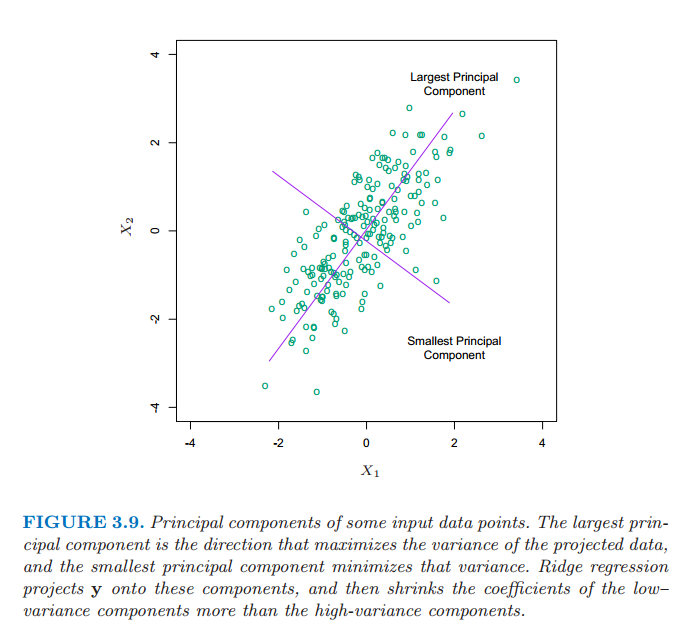
\includegraphics{C:/Users/YuQiFeng/Desktop/acadmeic files/2021-6-1/2021-6-1/fig1.png}
\end{frame}

\begin{frame}
我们定义有效自由度为: \[
\begin{aligned}
\operatorname{df}(\lambda) &=\operatorname{tr}\left[\mathbf{X}\left(\mathbf{X}^{\mathbf{T}} \mathbf{X}+\lambda \mathbf{I}\right)^{-1} \mathbf{X}^{T}\right] \\
&=\operatorname{tr}\left(\mathbf{H}_{\lambda}\right) \\
&=\sum_{j=1}^{p} \frac{d_{j}^{2}}{d_{j}^{2}+\lambda}
\end{aligned}
\tag{10}
\] 上面 \(\lambda\) 的单调递减函数是岭回归拟合的 \textbf{有效自由度
(effective degrees of freedom)}.通常在含 \(p\)
个变量的线性回归拟合中,拟合的自由度为
\(p\),也就是无约束参数的个数.这里想法是尽管岭回归拟合中所有的 \(p\)
个系数都不为 0,但是它们在由 \(\lambda\) 控制的约束下拟合.注意到当
\(\lambda=0\)(没有正则化)时 \(\df(\lambda)=p\),并且当
\(\lambda\rightarrow \infty\) 时
\(df(\lambda)\rightarrow 0\).当然总是对于截距总有一个额外的自由度,事先
(apriori) 已经去掉了。
\end{frame}

\hypertarget{lasso}{%
\section{\texorpdfstring{\emph{LASSO}}{LASSO}}\label{lasso}}

\begin{frame}[fragile]{\emph{LASSO}}
\[
\begin{align}
\hat{\beta}^{lasso}&=\underset{\beta}{\arg\min}\sum\limits_{i=1}^N(y_i-\beta_0-\sum\limits_{j=1}^px_{ij}\beta_j)^2\notag\\
&\text{subject to }\sum\limits_{j=1}^p\vert\beta_j\vert\le t 
\end{align}
\tag{11}
\]

我们也可以把\texttt{lasso}写成拉格朗日形式。 \[
\hat{\beta}^{lasso}=\underset{\beta}{\arg\min}\Big\{\sum\limits_{i=1}^N(y_i-\beta_0-\sum\limits_{j=1}^px_{ij}\beta_j)^2+\lambda\sum\limits_{j=1}^p\vert\beta_j\vert\Big\}\tag{3.52}\label{3.52}
\]
\end{frame}

\end{document}
